% A opção twoside (frente-e-verso) significa que a aparência das páginas pares
% e ímpares pode ser diferente. Por exemplo, as margens podem ser diferentes ou
% os números de página podem aparecer à direita ou à esquerda alternadamente.
% Mas nada impede que você crie um documento "só frente" e, ao imprimir, faça
% a impressão frente-e-verso.
%
% Aqui também definimos a língua padrão do documento (a última da lista) e
% línguas adicionais. Para teses do IME, no mínimo português e inglês são
% obrigatórios, porque independentemente da língua principal do texto é
% preciso fornecer o resumo nessas duas línguas. LaTeX aceita alguns nomes
% diferentes para a língua portuguesa; dentre as opções, prefira sempre
% "brazilian" para português brasileiro e "portuguese" para português europeu.
\documentclass[a4paper,12pt,twoside,brazilian,english,leqno]{book}
%\documentclass[a4paper,12pt,twoside,english,brazilian]{book}

\usepackage{packages/imegoodies}
\usepackage[thesis]{packages/imelooks}

\graphicspath{{fig/},{logos/},{img/},{images/},{imagens/}}

% Comandos rápidos para mudar de língua:
% \en -> muda para o inglês
% \br -> muda para o português
% \texten{blah} -> o texto "blah" é em inglês
% \textbr{blah} -> o texto "blah" é em português
\babeltags{br = brazilian, en = english}


%%%%%%%%%%%%%%%%%%%%%%%%%%%%%%%%%%%%%%%%%%%%%%%%%%%%%%%%%%%%%%%%%%%%%%%%%%%%%%%%
%%%%%%%%%%%%%%%%%%%%%%%%%%%%%%%%%% METADADOS %%%%%%%%%%%%%%%%%%%%%%%%%%%%%%%%%%%
%%%%%%%%%%%%%%%%%%%%%%%%%%%%%%%%%%%%%%%%%%%%%%%%%%%%%%%%%%%%%%%%%%%%%%%%%%%%%%%%

% O arquivo com os dados bibliográficos para biblatex; você pode usar
% este comando mais de uma vez para acrescentar múltiplos arquivos
\addbibresource{bibliografia.bib}

% Este comando permite acrescentar itens à lista de referências sem incluir
% uma referência de fato no texto (pode ser usado em qualquer lugar do texto)
%\nocite{bronevetsky02,schmidt03:MSc, FSF:GNU-GPL, CORBA:spec, MenaChalco08}
% Com este comando, todos os itens do arquivo .bib são incluídos na lista
% de referências
%\nocite{*}

% É possível definir como determinadas palavras podem (ou não) ser
% hifenizadas; no entanto, a hifenização automática geralmente funciona bem
\babelhyphenation{documentclass latexmk soft-ware clsguide} % todas as línguas
\babelhyphenation[brazilian]{Fu-la-no}
\babelhyphenation[english]{what-ever}

\title{Algebraic algorithm for maximum matching}[Algebraic algorithm for maximum matching]
\translatedtitle{Emparelhamento máximo}[Algoritmo algébrico para emparelhamento máximo]

\author{Antonio Marcos Shiro Arnauts Hachisuca}

\orientador{Prof. Dr. Marcel Kenji de Carli Silva}

\banca{
  \profa{} \dra{} Fulana de Tal (orientadora) -- IME-USP [sem ponto final],
  % Em inglês, não há o "ª"
  %Prof. Dr. Fulana de Tal (advisor) -- IME-USP [sem ponto final],
  Prof. Dr. Ciclano de Tal -- IME-USP [sem ponto final],
  \profa{} \dra{} Convidada de Tal -- IMPA [sem ponto final],
}

% A página de rosto da versão para depósito (ou seja, a versão final
% antes da defesa) deve ser diferente da página de rosto da versão
% definitiva (ou seja, a versão final após a incorporação das sugestões
% da banca).
\tipotese{
  tcc,
  programa={Ciência da Computação},
}

\defesa{
  local={São Paulo},
  data=2024-01-01, % YYYY-MM-DD
}

% A licença do seu trabalho. Use CC-BY, CC-BY-NC, CC-BY-ND, CC-BY-SA,
% CC-BY-NC-SA ou CC-BY-NC-ND para escolher a licença Creative Commons
% correspondente (o sistema insere automaticamente o texto da licença).
% Se quiser estabelecer regras diferentes para o uso de seu trabalho,
% converse com seu orientador e coloque o texto da licença aqui, mas
% observe que apenas TCCs sob alguma licença Creative Commons serão
% acrescentados ao BDTA. Se você tem alguma intenção de publicar o
% trabalho comercialmente no futuro, sugerimos a licença CC-BY-NC-ND.
%
%\direitos{CC-BY-NC-ND}
%
%\direitos{Autorizo a reprodução e divulgação total ou parcial deste
%          trabalho, por qualquer meio convencional ou eletrônico,
%          para fins de estudo e pesquisa, desde que citada a fonte.}
%
%\direitos{I authorize the complete or partial reproduction and disclosure
%          of this work by any conventional or electronic means for study
%          and research purposes, provided that the source is acknowledged.}
%
\direitos{CC-BY}

% Para gerar a ficha catalográfica, acesse https://fc.ime.usp.br/,
% preencha o formulário e escolha a opção "Gerar Código LaTeX".
% Basta copiar e colar o resultado aqui.
\fichacatalografica{}

% Configurações para teoremas, definições, etc.
\usepackage{mdframed}

\setlist{itemsep=0.5pt, parsep=0pt, topsep=0pt, partopsep=0pt}

%%%%%%%%%%%%%% Definitions %%%%%%%%%%%%%%%%%%%%%%
\newcommand{\Naturals}{\mathbb{N}}
\newcommand{\Integers}{\mathbb{Z}}
\newcommand{\Reals}{\mathbb{R}}
\newcommand*{\symdiff}{\mathbin{\Delta}}

\newcommand{\SC}[1]{\textsc{#1}}

\newmdenv[linecolor=black,linewidth=1pt]{problembox}

\newenvironment{problem}[1]
{
    \begin{problembox}
    \begin{center}
        \Large\SC{#1}
    \end{center}
	\itshape
	\noindent
}
{
    \end{problembox}
}

\newcommand\numberthis{\addtocounter{equation}{1}\tag{\theequation}}

%%%%%%%%%%%%% Theorems, lemmas, etc. %%%%%%%%%%%%

% Hints
% \newtheoremstyle{maybe} % nome do estilo
% {3pt} % espaço antes
% {3pt} % espaço depois
% {\itshape} % fonte do corpo
% {} % Indentação
% {\bfseries} % fonte do título
% {:} % pontuação após o título
% {.5em} % espaço após o título
% {\thmname{#1}\space(?)\thmnumber{ #2}\thmnote{ (#3)}} % formato do título
% % vazio significa {\thmname{#1}\thmnumber{ #2}\thmnote{ (#3)}}
\newtheorem{theorem}{Theorem}[section]

% Lemma style
\newtheorem{lemma}[theorem]{Lemma}

%% Definition style
\newtheorem{definition}[theorem]{Definition}

% Corollary style
\newtheorem{corollary}[theorem]{Corollary}

% Fact style
\newtheorem{fact}[theorem]{Fact}
\newtheorem*{fact*}{Fact}

% Proof style
\makeatletter
\renewenvironment{proof}[1][\proofname]{\par
  \pushQED{\qed}%
  \normalfont \topsep0pt \partopsep0pt % Removes extra vertical space before proof
  \trivlist
  \item[\hskip\labelsep
        \itshape
    #1\@addpunct{.}]\ignorespaces
}{%
  \popQED\endtrivlist\@endpefalse
}
\makeatother

\BeforeBeginEnvironment{theorem}{\vspace{0.4\baselineskip}}
\BeforeBeginEnvironment{lemma}{\vspace{0.4\baselineskip}}
\BeforeBeginEnvironment{fact}{\vspace{0.4\baselineskip}}
\BeforeBeginEnvironment{proposition}{\vspace{0.4\baselineskip}}
\BeforeBeginEnvironment{corollary}{\vspace{0.4\baselineskip}}
\BeforeBeginEnvironment{definition}{\vspace{0.4\baselineskip}}
\BeforeBeginEnvironment{example}{\vspace{0.4\baselineskip}}
\BeforeBeginEnvironment{remark}{\vspace{0.4\baselineskip}}

\begin{document}

%%%%%%%%%%%%%%%%%%%%%%%%%%% CAPA E PÁGINAS INICIAIS %%%%%%%%%%%%%%%%%%%%%%%%%%%%

% Aqui começa o conteúdo inicial que aparece antes do capítulo 1, ou seja,
% página de rosto, resumo, sumário etc. O comando frontmatter faz números
% de página aparecem em algarismos romanos ao invés de arábicos e
% desabilita a contagem de capítulos.
\frontmatter

\pagestyle{plain}

\onehalfspacing % Espaçamento 1,5 na capa e páginas iniciais

\maketitle % capa e folha de rosto

%%%%%%%%%%%%%%%% DEDICATÓRIA, AGRADECIMENTOS, RESUMO/ABSTRACT %%%%%%%%%%%%%%%%%%

\begin{dedicatoria}
Esta seção é opcional e fica numa página separada; ela pode ser usada para
uma dedicatória ou epígrafe.
\end{dedicatoria}

% Reinicia o contador de páginas (a próxima página recebe o número "i") para
% que a página da dedicatória não seja contada.
\pagenumbering{roman}

% Agradecimentos:
% Se o candidato não quer fazer agradecimentos, deve simplesmente eliminar
% esta página. A epígrafe, obviamente, é opcional; é possível colocar
% epígrafes em todos os capítulos. O comando "\chapter*" faz esta seção
% não ser incluída no sumário.
\chapter*{Agradecimentos}
\epigrafe{Do. Or do not. There is no try.}{Mestre Yoda}

Texto texto texto texto texto texto texto texto texto texto texto texto texto
texto texto texto texto texto texto texto texto texto texto texto texto texto
texto texto texto texto texto texto texto texto texto texto texto texto texto
texto texto texto texto. Texto opcional.

%%%%%%%%%%%%%%%%%%%%%%%%%%% LISTAS DE FIGURAS ETC. %%%%%%%%%%%%%%%%%%%%%%%%%%%%%

% Como as listas que se seguem podem não incluir uma quebra de página
% obrigatória, inserimos uma quebra manualmente aqui.
\cleardoublepage

\newcommand\disablenewpage[1]{{\let\clearpage\par\let\cleardoublepage\par #1}}

% Nestas listas, é melhor usar "raggedbottom" (veja basics.tex). Colocamos
% a opção correspondente e as listas dentro de um grupo para ativar
% raggedbottom apenas temporariamente.
\bgroup
\raggedbottom

%%%%% Listas criadas manualmente

%\chapter*{Lista de abreviaturas}
\disablenewpage{\chapter*{Lista de abreviaturas}}

\begin{tabular}{rl}
%  ABNT & Associação Brasileira de Normas Técnicas\\
   URL & Localizador Uniforme de Recursos (\emph{Uniform Resource Locator})\\
   IME & Instituto de Matemática e Estatística\\
   USP & Universidade de São Paulo
\end{tabular}

%\chapter*{Lista de símbolos}
\disablenewpage{\chapter*{Lista de símbolos}}

\begin{tabular}{rl}
%  $\omega$ & Frequência angular\\
%    $\psi$ & Função de análise \emph{wavelet}\\
%    $\Psi$ & Transformada de Fourier de $\psi$\\
\end{tabular}

% Quebra de página manual
\clearpage

%%%%% Listas criadas automaticamente

% Você pode escolher se quer ou não permitir a quebra de página
%\listoffigures
\disablenewpage{\listoffigures}

% Você pode escolher se quer ou não permitir a quebra de página
%\listoftables
\disablenewpage{\listoftables}

\disablenewpage{\listof{program}{\programlistname}}

% Sumário (obrigatório)
\tableofcontents

\egroup % Final de "raggedbottom"

% Referências indiretas ("x", veja "y") para o índice remissivo (opcionais,
% pois o índice é opcional). É comum colocar esses itens no final do documento,
% junto com o comando \printindex, mas em alguns casos isso torna necessário
% executar texindy (ou makeindex) mais de uma vez, então colocar aqui é melhor.
\index{Inglês|see{Língua estrangeira}}
\index{Figuras|see{Floats}}
\index{Tabelas|see{Floats}}
\index{Código-fonte|see{Floats}}
\index{Subcaptions|see{Subfiguras}}
\index{Sublegendas|see{Subfiguras}}
\index{Equações|see{Modo matemático}}
\index{Fórmulas|see{Modo matemático}}
\index{Rodapé, notas|see{Notas de rodapé}}
\index{Captions|see{Legendas}}
\index{Versão original|see{Tese/Dissertação, versões}}
\index{Versão corrigida|see{Tese/Dissertação, versões}}
\index{Palavras estrangeiras|see{Língua estrangeira}}
\index{Floats!Algoritmo|see{Floats, ordem}}


%%%%%%%%%%%%%%%%%%%%%%%%%%%%%%%% CAPÍTULOS %%%%%%%%%%%%%%%%%%%%%%%%%%%%%%%%%%%%%

% Aqui vai o conteúdo principal do trabalho, ou seja, os capítulos que compõem
% a dissertação/tese. O comando mainmatter reinicia a contagem de páginas,
% modifica a numeração para números arábicos e ativa a contagem de capítulos.
\mainmatter

\pagestyle{mainmatter}

% Espaçamento simples
\singlespacing

% A introdução não tem número de capítulo, então os cabeçalhos também não
\pagestyle{unnumberedchapter}
\chapter**{Introduction}
\label{cap:introduction}

\enlargethispage{.5\baselineskip}

Something.

\pagestyle{mainmatter}
\renewcommand*{\proofname}{Proof}

\chapter{Preliminaries}

The purpose of this chapter is to introduce key concepts related to the maximum matching algorithm. 
The chapter covers important topics such as the definition of graph maximum matching, the Sherman-Morrison-Woodbury formula, and the Schur complement. 
These concepts are fundamental for understanding the algorithm's correctness and time complexity.

\enlargethispage{.5\baselineskip}

\section{Graph theory}
\label{sec:graph}

\begin{definition}[Graph]
	\label{def:graph}
	A \textbf{graph} \(G\) is a triple \((V, E, \varphi)\) such that
	\begin{enumerate}[label=(\roman*)]
		\item \(V\) is the \textbf{vertex set};
		\item \(E\) is the \textbf{edge set};
		\item \(\varphi: E \to V \times V\) is a relation between each edge and a pair of vertices, called the \textbf{incidence function} of \(G\).
	\end{enumerate}
	Usually, it is used 
	\(V(G)\) or \(V_G\) to denote \(V\) and 
	\(E(G)\) or \(E_G\) to denote \(E\).
	Also, if \(e \in E(G)\) and \(\varphi(e) = (u, v)\), then \(u\) and \(v\) are the \textbf{ends} of \(e\);
	When the context is clear, \((u, v)\) may be abbreviated to \(uv\).
\end{definition}

\begin{definition}[Matching]
	\label{def:matching}
	For a graph \(G \coloneqq (V, E, \varphi)\), a set \(M \subseteq E\) is a \textbf{matching} of \(G\) if and only if no two edges in \(M\) share an end.
	A vertex \(v \in V\) is \(M\)-covered if some edge of \(M\) incides in \(v\), 
	and it is said that \(M\) covers \(v\);
	Otherwise, \(v\) is \(M\)-exposed.
	A matching \(M\) is:
	\begin{itemize}
		\item 
			\textbf{maximal}, if there is no edge \(e \in E \setminus M\) such that \(M \cup \{e\}\) is a matching of \(G\);

		\item
			\textbf{maximum}, if for every matching \(M'\) of \(G\) one has \(|M| \geq |M'|\);
	
		\item
			\textbf{perfect}, if \(2|V_G| = |M|\), i.e., every vertex of \(G\) is covered.
	\end{itemize}
	Now, the following problem can be introduced.
	\\
\end{definition}
\begin{problem}{Maximum matching}
	Given a graph, find a maximum matching of this graph.
\end{problem}
\section{Linear algebra}
\label{sec:linear_algebra}

% \begin{definition}[Fields]
% \label{def:fields}
% A \textbf{field} is a set with two binary operations on \(\mathbb{F}\) called \textit{addition} and \textit{multiplication}.
% The addition of two elements \(a\) and \(b\) from \(\mathbb{F}\) is denoted as \(a + b\).
% The multiplication of two elements \(a\) and \(b\) from \(\mathbb{F}\) is denoted as \(a \cdot b\).
% These operations must satisfy the following properties:
% \begin{enumerate}
%     \item Associativity: \(a + (b + c) = (a + b) + c\) and \(a \cdot (b \cdot c) = (a \cdot b) \cdot c\);
%     \item Commutativity: \(a + b = b + a\) and \(a \cdot b = b \cdot a\);
%     \item Additive and multiplicative identity: there exists two elements \(0\) and \(1\) in \(\mathbb{F}\) such that \(a + 0 = a\) and \(a \cdot 1 = a\);
%     \item Additive inverse: there exists an element \(-a\) such that \(a + (-a) = 0\);
%     \item Multiplicative inverse: there exists an element \(a^{-1}\) such that \(a \cdot a^{-1} = 1\);
%     \item Distributivity: 
% \end{enumerate}
% \end{definition}

\begin{definition}[Submatrix]
    Let \(M\) be a matrix, we say that \(M'\) is a \textbf{submatrix} of \(M\) if we can obtain \(M'\) by removing zero or more rows and/or columns from \(M\).
\end{definition}
\noindent
Let \(M\) be a matrix. 
For any sets of indices \(R\) and \(C\), we write \(M_{R,C}\) or \(M[R,C]\) to denote the submatrix of \(M\) formed by keeping only the rows indexed by \(R\) and columns indexed by \(C\). 
Furthermore, we use \(M[R,*]\) or \(M_{R, *}\) to represent the submatrix containing all rows indexed by \(R\) and all columns of \(M\) (resp., \(M[*, C]\)).
% \begin{definition}[Matrix inverse]
%     Let \(M\) be a matrix. 
%     The \textbf{inverse} of \(M\), denoted as \(M^{-1}\), is a matrix such that \(MM^{-1} = I\)
% \end{definition}
% 
% \begin{definition}[Singular matrix]
%     A matrix \(M\) is \textbf{singular} if it does not have an inverse.
%     A matrix is \textbf{non-singular} if it is not singular.
% \end{definition}

\begin{definition}[Schur complement]
    \label{def:schur}
    Let \(M\) be a square matrix of the form
    \[
        M =
        \begin{pmatrix}
            A & B \\
            C & D
        \end{pmatrix}
    \]
    where \(D\) is a square matrix; Then, if \(D\) is non-singular, the matrix \(A - B D^{-1} C\) is the \textbf{Schur complement} of \(D\) in \(M\).
    The Schur complement has the following properties:
    \begin{enumerate}
      \item \(\det(M) = \det(D)\det(A - BD^{-1}C)\).
    \end{enumerate}
\end{definition}

\begin{theorem}[Sherman-Morrison-Woodbury formula]
\label{thm:smw-formula}
  Suppose that \(M\) is non-singular. 
  Then
  \begin{enumerate}[label = (\arabic*)]
      \item \(M + UV^T\) is non-singular if and only if \(I + V^TM^{-1}U\) is non-singular;
      \item If \(M + UV^T\) is non-singular, then
      \[
          (M + UV^T)^{-1} = M^{-1} - M^{-1}U(I + V^TM^{-1}U)^{-1}V^TM^{-1}.
      \]
  \end{enumerate}
\end{theorem}

\begin{proof}
    For (1), let 
    \[
      A \coloneqq \begin{bmatrix} I & V^T \\ -U & M \end{bmatrix}.
    \]
    Note that the Schur complement of the block \(M\) of the matrix \(A\) is \(I + V^TM^{-1}U\) and that 
    \[
      \begin{bmatrix} I & V^T \\ -U & M \end{bmatrix} = 
      \begin{bmatrix} I & 0 \\ -U & I \end{bmatrix} \begin{bmatrix} I & V^T \\ 0 & M + UV^T \end{bmatrix}.
    \]
    Then, one has
    \begin{align*}
      \det(M)\det(I + V^TM^{-1}U) 
      &= \det(A) \\
      &= \det\bigg(\begin{bmatrix} I & 0 \\ -U & I \end{bmatrix} \begin{bmatrix} I & V^T \\ 0 & M + UV^T \end{bmatrix}\bigg) \\
      &= \det(I) \det(M+UV^T) = \det(M+UV^T).
    \end{align*}
    Thus, (1) is proven.
    For (2), it suffices to verify that 
    \[
        (M + UV^T)(M^{-1} - M^{-1}U(I + V^TM^{-1}U)^{-1}V^TM^{-1}) = I.
    \]
    Let \(A \coloneqq (I + V^TM^{-1}U)\), then
    \begin{align*}
        &\!\!\!\!\!\!\!\!\!\!\!\!\!\!\!\!\!\! (M + UV^T)(M^{-1} - M^{-1}U(I + V^TM^{-1}U)^{-1}V^TM^{-1})\\
        = \, &(M + UV^T)(M^{-1} - M^{-1}UA^{-1}V^TM^{-1})\\
        = \, &(I - UA^{-1}V^TM^{-1}) + (UV^TM^{-1} - UV^TM^{-1}UA^{-1}V^TM^{-1}) \\
        = \, &(I + UV^TM^{-1}) - (UA^{-1}V^TM^{-1} + UV^TM^{-1}UA^{-1}V^TM^{-1}) \\
        = \, &(I + UV^TM^{-1}) - U(I + V^TM^{-1}U)(A^{-1}V^TM^{-1}) \\
        = \, &(I + UV^TM^{-1}) - UAA^{-1}V^TM^{-1} \\
        = \, &I + UV^TM^{-1} - UV^TM^{-1} = I. \qedhere \\
    \end{align*}
\end{proof}

\begin{corollary}[{\citet[Corollary 2.1]{Harvey:Paper}}]
    \label{cor:update_cor} 
    Let \(M\) be a non-singular square matrix, let \(N \coloneqq M^{-1}\) and let \(S\) be a subset of rows from \(M\).
    Let \(\tilde{M}\) be a matrix that which is identical to \(M\) except that \(\tilde{M}_{S, S} \neq M_{S, S}\)
    and \(\Delta \coloneqq \tilde{M}_{S, S} - M_{S, S}\).
    If \(\tilde{M}\) is non-singular, then
    \[
        \tilde{M}^{-1} = N - N_{*, S}(I + \Delta N_{S, S})^{-1}\Delta N_{S, *}.
    \]
\end{corollary}

\begin{proof}
    Let \(k \coloneqq |S|\). 
    Let \(U\)\footnote{Every column should be a canonical basis vector from \(S\)} be a \(n \times k\) matrix that selects the \(S\) columns from a \(n \times n\) matrix, i.e.
    for a \(n \times n\) matrix \(M\), one has \(MU = M_{*, S}\). Let \(V^T \coloneqq \Delta U^T\). 
    Then, by \cref{thm:smw-formula}, 
    \begin{align*}
        \tilde{M}^{-1} &= (M + U V^T)^{-1} \\
        &= N - N U (I + \Delta U^T N U)^{-1} \Delta U^T N \\
        &= N - N_{*, S} (I + \Delta U^T N U)^{-1} \Delta N_{S, *} \\
        &= N - N_{*, S} (I + \Delta N_{S, S})^{-1} \Delta N_{S, *}. \qedhere
    \end{align*}
\end{proof}

\begin{definition}[Skew-symmetric matrix]
\label{def:skew}
    A matrix \(M\) is \textbf{skew-symmetric} if \(M = -M^{T}\).
\end{definition}

\begin{fact}[Inverse of a skew-symmetric matrix]
    Let \(M\) be a skew-symmetric matrix.
    If \(M\) is non-singular, then \(M^{-1}\) is also skew-symmetric.
\end{fact}

\section{Matrix Algorithms}
\label{matrix:time_complexity}

% This section presents the matrix algorithms used throughout this paper.

\begin{definition}[Matrix multiplication exponent]
  The \textbf{matrix exponent multiplication exponent}, denoted by \(\omega\), is the infimum of the exponent over all matrix multiplication algorithms.
  That is there is a known algorithm that solves matrix multiplication in \(O(n^{\omega + o(1)})\) field operations.
\end{definition}

\noindent
The following milestones related to matrix multiplication algorithms were found:
\begin{center}
  \begin{tabular}{|c|c|c|}
    \hline
    Year & Author(s) & Bound on omega \\
    \hline
    1969 & \citet{Strassen1969} & 2.8074 \\ 
    1990 & \citet{COPPERSMITH1990} & 2.3755 \\
    2024 & \citet{2024asymmetryyieldsfastermatrix} & 2.371339 \\
    \hline
  \end{tabular}
\end{center}

\noindent
The following algorithms can be done in \(O(n^\omega)\):

\begin{enumerate}
  \item \textbf{Matrix inversion}, see \citet[Theorem 28.2]{CLRS}; 
  \item \textbf{Matrix rank}, see (TODO: add citation).
\end{enumerate}


\chapter{Perfect matching}

\section{Tutte Matrix}

\begin{definition}[Indeterminates]

\end{definition}

\begin{definition}[Tutte Matrix]
\label{def:tutte_matrix}
    Let \(G\) be a graph and \(n \coloneqq |V_G|\).
    For each edge \(\{u,v\} \in E_G\) associate an indeterminate \(t_{\{u,v\}}\).
    The Tutte matrix is the \(n \times n\) skew-symmetric matrix such that \(T_{u,v} = \pm t_{\{u, v\}}\) if \(\{u,v\} \in E_G\) and \(0\), otherwise.
    The sign is chosen such that \(T\) is skew-symmetric.
    The Tutte matrix of \(G\) is denoted as \(T_G\).
\end{definition}

For a Tutte matrix \(T\), its Pfaffian, denoted \(Pf(T)\), is a polynomial whose complete mathematical definition involves sophisticated algebraic concepts beyond our current scope. 
However, two fundamental properties of the Pfaffian are crucial:
\begin{enumerate}
    \item The Pfaffian \(Pf(T)\) equals the number of perfect matchings in the underlying graph of \(T\);
    \item There exists a fundamental relationship between the Pfaffian and the determinant of a Tutte matrix: \(\det(T) = Pf(T)^2\). 
\end{enumerate}

For a comprehensive treatment of this remarkable polynomial and its properties, we refer the reader to Chapter 7 of \cite{Godsil:1993}.

\begin{fact}[Tutte matrix perfect matching condition]
    \label{fact:matching_condition}
    A graph \(G\) has a perfect matching iff \(T_G\) is non-singular.
\end{fact}

\begin{proof}
    Direct from the property \(\det(T) = Pf(T)^2\).
\end{proof}

While this property of Tutte matrices is powerful, it presents a computational challenge for algorithmic applications. 
The issue stems from the relationship \(\det(T) = Pf(T)^2\), where \(Pf(T)\) contains a term for each perfect matching in graph (G). 
Since a graph may contain exponentially many perfect matchings, direct computation becomes infeasible.

\subsection{Probabilistic representation of a Tutte Matrix}
A breakthrough came from \cite{Lovasz:Random}, who demonstrated a probabilistic solution: If we replace the non-zero entries of (T) with random values from a sufficiently large field, the matrix's rank is preserved with \textbf{high} probability. 
This provides a computationally feasible approach.

\begin{lemma}[Schwartz-Zippel]
\label{lemma:schwartz-zippel}
    \textbf{[Find the reference itself]}
    Should state that if we evaluate this polynomial at a random point in \(F^{|E|}_q\), then the evaluation is zero with probabilty at most \(n/q\).
    That is something non-zero in indeterminates is zero with random values with probabily at most \(n/q\).
\end{lemma}

\begin{proof}
    Reference Schwartz-Zippel lemma.
\end{proof}

According to \cref{lemma:schwartz-zippel}, selecting a sufficiently large field significantly reduces the probability of failure.
Constructing such a field is straightforward. 
For any prime number \(p\), the set of integers modulo \(p\), denoted as \(\Integers_{p}\), forms a field of size \(p\).

% A tutte matrix to refer to randomized tutte matrix

\section{Naive algorithm}

Using \cref{fact:matching_condition}, the following algorithm finds a perfect matching in time \(O(n^{\omega+2})\).
\begin{programruledcaption}{\(\SC{NaiveAlgorithm}\)}
    \begin{lstlisting}[
      language={pseudocode},
      style=pseudocode,
      style=wider,
      functions={},
      specialidentifiers={},
    ]
        function NaiveAlgorithm(G)
            for \textbf{ each } $e \in E_G$ do
                $G'$ := $(V_G, E_G \setminus \{e\})$
                if $T_{G'}$ is singular then // By \cref{fact:matching_condition}, edge $e$ is inessential.
                    $G$ := $G'$ 
                end
            end
            return $E_G$ // Only the essential edges remain in $G$.
        end
    \end{lstlisting}
\end{programruledcaption}
\noindent
Let \(f(n)\) be the running time of \(\SC{NaiveAlgorithm}\) when \(|V_G| \eqcolon n\).
The running time can be expressed as:
\[
    f(n) = \binom{n}{2} O(n^\omega) = O(n^2) O(n^\omega) = O(n^{\omega+2}).
\]

\section{Rank-two update algorithm}

The bottleneck of the previous algorithm is the necessity to recompute the whole matrix inverse after each iteration.

\begin{theorem}[Rank-two update]
\label{thm:rank-two}
    Let \(G\) be a graph, \(N \coloneqq T_G^{-1}\) and \(S \subseteq V_G\) such that \(|S| = 2\). 
    Let \(\tilde{T}\) be a matrix which is identical to \(T_G\) except that \(\tilde{T}_{S, S} = 0\).
    If \(\tilde{T}\) is non-singular, then
    \[
        \tilde{T}^{-1} \coloneqq N + N_{*, S} \cdot 
        \begin{pmatrix}
            1 / (1 + T_{u, v}N_{u, v}) & 0 \\
            0 &  1 / (1 + T_{v, u}N_{v, u})
        \end{pmatrix}
        \cdot T_{S, S} \cdot N_{S, *}.
    \]
\end{theorem}

\begin{proof}
TODO: amsah - Prove \((I - T_{S, S}N_{S, S})^{-1} = 
        \begin{pmatrix}
            1 / (1 + T_{\{u, v\}}N_{\{u, v\}}) & 0 \\
            0 &  1 / (1 + T_{\{v, u\}}N_{\{v, u\}})
        \end{pmatrix} \)
\end{proof}

\begin{corollary}[Edge removal condition]
    \label{cor:condition_edge_removal}
    Let \(G\) be a graph, \(T\) be the Tutte matrix of \(G\) and \(N \coloneqq T^{-1}\).
    An edge \(ij\) is essential if and only if \(N_{ij} = -1/T_{ij}\).
\end{corollary}

\begin{proof}
    TODO(amsah): equation (3.6) shows this necessity.
\end{proof}

We use \cref{cor:condition_edge_removal} to quickly decide if an edge is essential. 
If it's not, we remove it and update the matrix using a rank-2 update. 
This removes the necessity to recompute the whole inverse in each iteration.

\begin{programruledcaption}{\(\SC{Rank-2 update algorithm}\)}
    \begin{lstlisting}[
      language={pseudocode},
      style=pseudocode,
      style=wider,
      functions={Rank2Update},
      specialidentifiers={},
    ]
        function Rank2Update(S, T, N) // $|S| = 2$
            return $N + N_{*, S} \cdot \begin{pmatrix} 1 / (1 + T_{u, v}N_{u, v}) & 0 \\ 0 & 1 / (1 + T_{v, u}N_{v, u})\end{pmatrix} \cdot  T_{S, S} \cdot N_{S, *}$ // \cref{thm:rank-two}.
        end

        function Rank2Algorithm(G)
            $T$ := $T_G$
            $N$ := $T^{-1}$
            for \textbf{ each } $\{u,v\} \in E_G$ do
                if $N_{\{u,v\}} = - 1 / T_{\{u, v\}}$ then // \cref{cor:condition_edge_removal}
                    $N$ := Rank2Update($\{u, v\}, T, N$)
                    $T_{u, v}$ := 0
                    $T_{v, u}$ := 0
                end
            end
            return $E_G$ // Only the essential edges remain in $G$.
        end
    \end{lstlisting}
\end{programruledcaption}

First, let \(t(n)\) be the running time of \(\SC{Rank2Update}\) when \(|V_G| \eqcolon n\).
Let \(A\) be a \(n \times m\) matrix and let \(B\) be a \(m \times o\).
In this context, note that \(\tilde{N}T_{S, S}\) is a \(2 \times 2\) matrix.
Therefore, \(N_{*, S}\tilde{N}T_{S, S}\) is a \(n \times 2\) matrix.
Consequently,
\[
    t(n) = O(2n^2) = O(n^2).
\]

Let \(g(n)\) be the running time of \(\SC{Rank-2 update algorithm}\) when \(n \eqcolon |V_G|\).
The running time can be expressed as:
\begin{align*}
    g(n) = \binom{n}{2} t(n) = \binom{n}{2} O(n^2) = O(n^2) O(n^2) = O(n^4).
\end{align*}
\chapter{Harvey's algorithm}
\label{chap:harvey}

% \begin{enumerate}
%     \item Brief of the idea;
%     \item Pseudo-algorithm;
%     \item Corretude;
% \end{enumerate}
This chapter presents the probabilistic algorithm proposed by \citet{Harvey:Paper} that finds a perfect matching in general graphs with time complexity \(O(n^\omega)\).

\section{Algorithm}

The main bottleneck in the previous algorithm was the need to update the entire inverse matrix at each step. 
Harvey's algorithm addresses this limitation by employing a divide-and-conquer strategy combined with lazy updates. 
After each recursive step, only the necessary portions of the inverse matrix are updated.
As a result, Harvey's algorithm has a time complexity of \(O(n^\omega)\).

For a graph \(G\) and \(n = |V(G)|\). 
The algorithm maintains two matrices, \(T\) and \(N\), that are initialized as
\begin{enumerate}
    \item \(T \coloneqq \) a Tutte matrix where the entries were randomly chosen\footnote{\cref{sec:prob_tutte}};
    \item \(N \coloneqq T^{-1}\).
\end{enumerate}
It relies on two recursive functions: \(\SC{DeleteEdgesCrossing}\) and \(\SC{DeleteEdgesWithin}\). 

\subsection{\(\SC{DivideInTwo}\)}
\(\SC{DivideInTwo(A)}\) is a function that divides a set \(A\) in two parts, \(R\) and \(S\), such that \(R \cup S = A\), \(R \cap S = \emptyset\) and \(|R| - |S| \leq 1\).
This function has time complexity \(O(n)\) and can be implemented through integer indexing the set.

\subsection{\(\SC{DeleteEdgesCrossing}\)}

$\SC{DeleteEdgesCrossing}(R, S)$: receives two disjoint sets of vertices \(R\) and \(S\) and 
deletes inessential edges that connect a vertex in \(R\) to a vertex in \(S\).
The following invariant must be preserved:
\begin{itemize}
    \item \(\SC{DeleteEdgesCrossing}(R, S)\): initially has \(N_{R \cup S, R \cup S} = {T^{-1}}_{R \cup S, R \cup S}\) and this property is restored after each call 
    of \(\SC{DeleteEdgesCrossing}(R_i, S_j)\).
\end{itemize}
To maintain this invariant the following updates are done. 

\begin{theorem}[Update 1]
\label{update:1}
    Let \(R, S\) be two disjoint sets of vertices such that \(|R| = |S| = 1\).
    Let \(N \coloneqq T^{-1}\), \(r \in R\) and \(s \in S\).
    If \(\{r, s\}\) is inessential, let \(\tilde{T}\) be the Tutte matrix of \(G\) without edge \(\{r, s\}\), then one has
    \[
        \tilde{T}^{-1}_{R, S} = N_{R, S} (1 - T_{R, S} N_{R, S}) / (1 + T_{R, S} N_{R, S})
    \]
    and
    \[
        \tilde{T}^{-1}_{S, R} = N_{S, R} (1 - T_{S, R} N_{S, R}) / (1 + T_{S, R} N_{S, R}) = -\tilde{T}^{-1}_{R, S}.
    \]
\end{theorem}

\begin{proof}
  TODO
%    The inverse of a Tutte Matrix is skew-symmetric, thus \(N_{s, r} = -N_{r, s}\).
%    Let \(V \coloneqq R \cup S\)
%    By \cref{cor:update_cor}, one has:
%    \begin{align*}
%        {T'}^{-1}_{X, X} &= N_{X, X} - N_{X, X} (I + \Delta N_{X, X})^{-1} \Delta N_{X, X} \\
%        &= N_{X, X} - N_{X, X} \bigg(I + \begin{bmatrix} 0 & -T_{r, s} \\ -T_{s, r} & 0 \end{bmatrix} \begin{bmatrix} 0 & N_{r, s} \\ N_{s, r} & 0 \end{bmatrix}\bigg)^{-1} \Delta N_{X, X} \\ &= N_{X, X} - N_{X, X} \bigg(I + \begin{bmatrix} -T_{r, s} N_{s, r} & 0 \\ 0 & -T_{s, r} N_{r, s} \end{bmatrix} \bigg)^{-1} \Delta N_{X, X} \\
%        &= N_{X, X} - N_{X, X} \bigg(I + \begin{bmatrix} T_{r, s} N_{r, s} & 0 \\ 0 & T_{r, s} N_{r, s} \end{bmatrix} \bigg)^{-1} \Delta N_{X, X} \\
%        &= N_{X, X} - N_{X, X} \bigg(\begin{bmatrix} 1 + T_{r, s} N_{r, s} & 0 \\ 0 & 1 + T_{r, s} N_{r, s} \end{bmatrix} \bigg)^{-1} \Delta N_{X, X} \\
%        &= N_{X, X} - N_{X, X} \begin{bmatrix} \frac{1}{1 + T_{r, s} N_{r, s}} & 0 \\ 0 & \frac{1}{1 + T_{r, s} N_{r, s}} \end{bmatrix} \Delta N_{X, X} \\
%        &= N_{X, X} + N_{X, X} \begin{bmatrix} \frac{1}{1 + T_{r, s} N_{r, s}} & 0 \\ 0 & \frac{1}{1 + T_{r, s} N_{r, s}} \end{bmatrix} \begin{bmatrix} T_{r, s} N_{s, r} & 0 \\ 0 & T_{s, r} N_{r, s} \end{bmatrix} \\
%        &= N_{X, X} + N_{X, X} \begin{bmatrix} \frac{T_{r, s}N_{s, r}}{1 + T_{r, s} N_{r, s}} & 0 \\ 0 & \frac{T_{s, r}N_{r, s}}{1 + T_{r, s} N_{r, s}} \end{bmatrix} \\
%        &= N_{X, X} + \begin{bmatrix} 0 & N_{r, s} \\ N_{s, r} & 0 \end{bmatrix} \begin{bmatrix} \frac{T_{s, r}N_{r, s}}{1 + T_{r, s} N_{s, r}} & 0 \\ 0 & \frac{T_{r, s}N_{r, s}}{1 + T_{r, s} N_{r, s}} \end{bmatrix} \\
%        &= N_{X, X} + \begin{bmatrix} 0 & \frac{N_{r, s}T_{s, r}N_{s, r}}{1 + T_{r, s} N_{r, s}} \\ \frac{N_{s, r}T_{r, s}N_{s, r}}{1 + T_{r, s} N_{r, s}} & 0 \end{bmatrix} \\
%        &= \begin{bmatrix} 0 & N_{r, s} + \frac{N_{r, s}T_{s, r}N_{s, r}}{1 + T_{r, s} N_{r, s}} \\ N_{s, r} + \frac{N_{s, r}T_{r, s}N_{s, r}}{1 + T_{r, s} N_{r, s}} & 0 \end{bmatrix} \\ 
%        &= \begin{bmatrix} 0 & \frac{N_{r, s}(1 + T_{r, s}N_{r, s} + T_{s, r}N_{s, r})}{1 + T_{r, s} N_{r, s}} \\ N_{s, r} + \frac{N_{s, r}T_{r, s}N_{s, r}}{1 + T_{r, s} N_{r, s}} & 0 \end{bmatrix} \\ 
%        &= \begin{bmatrix} 0 & \frac{N_{r, s}}{1 + T_{r, s} N_{r, s}} \\ N_{s, r} + \frac{N_{s, r}T_{r, s}N_{s, r}}{1 + T_{r, s} N_{r, s}} & 0 \end{bmatrix}
%    \end{align*}
\end{proof}

\begin{theorem}[Update 2]
\label{update:2}
    Let \(R, S\) be two disjoint set of vertices. Let \(T'\) be \(T\) after removing some (possibly zero) edges from \(G\) with an end in \(R_i\) and another in \(S_j\).
    Then, let \(N := T^{-1}\) and \(\Delta := T' - T\), one has:
    \[
        {T'}^{-1}_{R \cup S, R \cup S} = N_{R \cup S, R \cup S} - N_{R \cup S, R_i \cup S_j}(I + \Delta N_{R_i \cup S_j, R_i \cup S_j})^{-1} \Delta N_{R_i \cup S_j, R \cup S}.
    \]
\end{theorem}

\begin{proof}
    Direct from \cref{cor:update_cor}. Update the whole matrix with \ref{cor:update_cor} and select only the desired submatrix.
\end{proof}

We have the following algorithm.

\begin{programruledcaption}{Harvey's algorithm: \(\SC{DeleteEdgesCrossing}\)}
    \begin{lstlisting}[
      language={pseudocode},
      style=pseudocode,
      style=wider,
      functions={DeleteEdgesCrossing, RemoveEdge, DivideInTwo},
      specialidentifiers={},
    ]
        function DeleteEdgesCrossing(R, S) // R and S are \textbf{disjoint} sets of vertices.
            if $|R| = 0$ or $|S| = 0$ then return // There are no edges.

            if $|R| = 1$ and $|S| = 1$ then // There is at most \textbf{one} edge.
                Let $r$ in $R$
                Let $s$ in $S$
                if $T_{r, s} \neq 0$ \textbf{ and } $N_{r, s} \neq -1 / T_{r, s}$ then // \cref{cor:condition_edge_removal}.
                    $N_{r, s}$ := $N_{r, s} (1 - T_{r, s} N_{r, s}) / (1 + T_{r, s} N_{r, s})$ // \cref{update:1}.
                    $N_{s, r}$ := $-N_{r, s}$
                    RemoveEdge($T, rs$)
                return

            $RS$ := $R \cup S$
            $R_1, R_2$ := DivideInTwo($R$)
            $S_1, S_2$ := DivideInTwo($S$)
            for i \textbf{in} {1, 2} do
                for j \textbf{in} {1, 2} do
                    $T', N'$ := $T, N$ // Save current T and N states
                    DeleteEdgesCrossing($R_i, S_j$)
                    $\Delta$ := $T_{R_i \cup S_j, R_i \cup S_j} - {T'}_{R_i \cup S_j, R_i \cup S_j}$
                    $N_{RS, RS}$ := $N_{RS, RS}' - {N'}_{RS, R_i \cup S_j} (I + \Delta {N'}_{R_i \cup S_j, R_i \cup S_j})^{-1} \Delta {N'}_{R_i \cup S_j, RS}$ // \cref{update:2}.
    \end{lstlisting}
\end{programruledcaption}

\subsubsection{Implementation}
\noindent
The C++ implementation is available at 
\href{https://github.com/antoniomsah/algebraic-max-matching/blob/main/code/algorithms/harvey-algorithm.hpp#L51}{//code/algorithms/harvey-algorithm.hpp:L51}.

\subsubsection{Time complexity}
\noindent
Let \(f(r, s)\) be the running time for \(\SC{DeleteEdgesCrossing}(R, S)\) when \(|R| = r\) and \(|S| = s\).
Let \(n = r + s\). The base cases are \(O(1)\).
Otherwise, a line-by-line analysis:
\begin{enumerate}
    \item \textbf{Dividing in half (Lines 16 and 17)}: Takes \(O(n)\) time;
    \item \textbf{Saving the states (Line 20)}: Takes \(O(n^2)\) time;
    \item \textbf{Recursive call (Line 21)}: Recurrence is \(f(r/2, s/2)\);
    \item \textbf{Delta (Line 22)}: Matrix subtraction is \(O(n^2)\);
    \item \textbf{Update submatrix (Line 23)}: Takes \(O(n^\omega)\).
\end{enumerate}
Combining these steps, we have
\begin{align*}
    f(r, s) &= O(1) + O(1) + O(n^2) + 4(O(n^2) + T(r / 2, s / 2) + O(n^\omega))  \\
    &= 4O(n^2) + 4f(r / 2, s / 2) + 4O(n^\omega) \\
    &= 4f(r / 2, s / 2) + 4O(n^\omega).
\end{align*}
Now, applying the master theorem for recursions, i.e. 
\[
  T(n) = aT(n/b) + f(n).
\]
In this case, \(T(n) = t(r, s)\), \(a = 4\), \(b = 2\) and \(f(n) = O(n^\omega)\), then if \(\omega > \log_{b}a = 2\) the complexity is dominated by \(O(n^\omega)\).
From \cref{matrix:time_complexity}, the best currently known matrix multiplication algorithm has \(\omega > 2\).
Thus, the complexity is dominated by \(O(n^\omega)\) and
\begin{equation}
  \label{alg:delcrossing}
  f(r, s) = 4f(r/2, s/2) + 4O(n^\omega) = 8O(n^\omega) = O(n^\omega). 
\end{equation}

\subsection{\(\SC{DeleteEdgesWithin}\)}

\(\SC{DeleteEdgesWithin}\): receives a set of vertices \(S\) and deletes inessential edges that have both ends in \(S\).
The following invariant must be preserved:
\begin{itemize}
    \item \(\SC{DeleteEdgesWithin}(S)\): initially has \(N_{S, S} = T^{-1}_{S, S}\) and this property is restored after each call of \(\SC{DeleteEdgesWithin}\)
    and \(\SC{DeleteEdgesCrossing}\).
\end{itemize}
To maintain this invariant the following update is done.
\begin{theorem}[Update 3]
\label{update:3}
    Let \(S \subseteq V_G\), \(T'\) be \(T\) after removing some (possibly zero) edges from \(G\) with both ends in \(S\).
    Then, let \(N \coloneqq T^{-1}\) and \(\Delta \coloneqq T' - T\), one has
    \[
        {T'}^{-1}_{S, S} = N_{S, S} - N_{S, S_i}(I + \Delta N_{S_i, S_i})^{-1} \Delta N_{S_i, S}.
    \]
\end{theorem}

\begin{proof}
    Direct from \cref{cor:update_cor}. Update the whole matrix with \ref{cor:update_cor} and select only the desired submatrix.
\end{proof}

We have the following algorithm.

\begin{programruledcaption}{Harvey's algorithm: \(\SC{DeleteEdgesWithin}\)}
    \begin{lstlisting}[
      language={pseudocode},
      style=pseudocode,
      style=wider,
      functions={DeleteEdgesCrossing, DeleteEdgesWithin, DivideInTwo},
      specialidentifiers={},
    ]
        function DeleteEdgesWithin(S)
            if |S| = 1 return

            $S_1, S_2$ := DivideInTwo($S, 2$)
            for i \textbf{in} {1, 2} do
                $T', N'$ := $T, N$ // Save current T and N states
                DeleteEdgesWithin($S_i$)
                $\Delta$ := $T_{S_i, S_i} - {T'}_{S_i, S_i}$
                $N_{S, S}$ := $N' - {N'}_{S, S_i}(I + \Delta {N'}_{S_i, S_i})^{-1} \Delta {N'}_{S_i, S}$ // \cref{update:3}. 
            DeleteEdgesCrossing($S_1, S_2$)
    \end{lstlisting}
\end{programruledcaption}

\subsubsection{Implementation}
\noindent
The C++ implementation is available at 
\href{https://github.com/antoniomsah/algebraic-max-matching/blob/main/code/algorithms/harvey-algorithm.hpp#L18}{//code/algorithms/harvey-algorithm.hpp:L18}.

\subsubsection{Time complexity}
\noindent
Let \(g(n)\) be the running time of \(\SC{DeleteEdgesWithin}(S)\) when \(|S| = n\).
The base case is direct.
Then, through a line-by-line analysis we have
\begin{enumerate}
  \item \textbf{DivideInTwo (Line 4)}: Takes \(O(n)\) times;
  \item \textbf{Saving the states (Line 6)}: Takes \(O(n^2)\) time;
  \item \textbf{Recursive call (Line 7)}: Takes \(g(n/2)\) time;
  \item \textbf{Delta (Line 8)}: Takes \(O(n^2)\);
  \item \textbf{Update 3 (Line 9)}: Takes \(O(n^\omega)\) time;
  \item \textbf{DeleteEdgesCrossing (Line 10)}: Takes \(f(n/2, n/2)\).
\end{enumerate}
Now, combining these steps:
\begin{align*}
    g(n) &= O(n) + 2 (2O(n^2) + g(n / 2) + O(n^\omega)) + f(n/2, n/2) &  \\
    &= O(n) + 2 (2O(n^2) + g(n / 2) + O(n^\omega)) + O(n^\omega) & \text{by \ref{alg:delcrossing}} \\
    &= 2g(n / 2) + 3O(n^\omega).
\end{align*}
Similarly to \cref{alg:delcrossing}, we have
\begin{equation}
\label{alg:delwithin}
  g(n) = 2g(n / 2) + 3O(n^\omega) = O(n^\omega).
\end{equation}

\subsection{\(\SC{PerfectMatching}\)}

\(\SC{PerfectMatching}\): Receives a graph \(G\) and finds a perfect matching, or returns \(\emptyset\) if one does not exist.
It creates a Tutte Matrix of \(G\) with random entries.
Note that calling \(\SC{DeleteEdgesWithin}(V(G))\) is equivalent to deleting every non-essential edge from \(G\).
Thus, after this call, the graph only has essential edges, i.e., edges from the perfect matching. 
Consequently, there is the following implementation:

\begin{programruledcaption}{Harvey's algorithm: \(\SC{Perfect Matching}\)}
    \begin{lstlisting}[
      language={pseudocode},
      style=pseudocode,
      style=wider,
      functions={DeleteEdgesWithin},
      specialidentifiers={},
    ]
        function PerfectMatching(G)
            T := $\SC{TutteMatrix}(G)$
            if T \textbf{ is singular} then return $\emptyset$ // The graph has no perfect matching
            N := $T^{-1}$
            DeleteEdgesWithin($V$)
            return $E(T)$
    \end{lstlisting}
\end{programruledcaption}

\subsubsection{Implementation}
\noindent
The C++ implementation is available at 
\href{https://github.com/antoniomsah/algebraic-max-matching/blob/main/code/solver.hpp#L89}{//code/solver.hpp:L89}.

\subsubsection{Time complexity}
\noindent
Let \(T(n)\) be the running time of \(\SC{PerfectMatching(G)}\) when \(|V| = n\). 
A line-by-line comparison:
\begin{enumerate}
  \item \textbf{Building a TutteMatrix (Line 2)}: Takes \(O(n^2)\) time;
  \item \textbf{Checking if a matrix is singular (Line 3)}: Takes \(O(n^\omega)\) time;
  \item \textbf{Calculating a matrix inverse (Line 4)}: Takes \(O(n^\omega)\) time;
  \item \textbf{DeleteEdgesWithin (Line 5)}: From \cref{alg:delwithin}, takes \(g(|V|) = O(n^\omega)\) time;
  \item \textbf{Returning the matching (Line 6)}: Takes \(O(n^2)\) time.
\end{enumerate}
Combining these steps, we have:
\begin{equation}
\label{alg:harvey_complexity}
    T(n) = O(n^2) + O(n^\omega) + O(n^\omega) + O(n^\omega) + O(n^2) = O(n^\omega).
\end{equation}

\subsubsection{Probability of failure}
\noindent
Let \(\delta\) be the probability of failure.
From \cref{lemma:schwartz-zippel}, deciding if an edge can be deleted fails with probability \(n / q\) where \(q\) is the size of the field. 
Since there are \(\binom{n}{2}\) edges, then 
\[
  \delta \leq \binom{n}{2} n / q < n^3 / q.
\]

\subsubsection{Corretude}
\noindent
To prove the algorithm's correctness, it suffices that for every edge \(uv \in E(G)\), when evaluating whether \(uv\) can be removed (using \cref{cor:condition_edge_removal}), one has \(N_{uv} = T^{-1}_{uv}\).
This equality is guaranteed by the invariants.
Since the updates ensure that the invariants are maintained throughout the algorithm, we can conclude that the edge removal decisions are correct.

\section{Analysis}

This section compares Harvey's algorithm with three perfect matching algorithms:
\begin{enumerate}
   \item The simple algorithm presented in \cref{alg:simple};
   \item The rank-two algorithm described in \cref{alg:rank-two};
 \item A graph theory-based implementation used in competitive programming competitions (see \href{https://codeforces.com/blog/entry/92339}{codeforces.com/blog/entry/92339}).
\end{enumerate}
The comparisons are made through random tests together with a verifier that asserts the output is a valid perfect matching.


\chapter{Extension to Maximum Matching}
\label{chap:maximum_matching}

This chapter shows how to extend the perfect matching algorithms to solve the maximum matching problem.

\section{Maximum Matching algorithm}

The extension to maximum matching is based on the following theorem by Lovasz.
\begin{theorem}[\citet{plummer1986matching}]
\label{thm:rank_matching}
    Let \(G\) be a graph and let \(T\) be the Tutte Matrix of \(G\).
    Then, \(\rank(T_G) = 2\nu(G)\).
\end{theorem}

\begin{proof}
  See \citet[p.~560]{Rabin1989}.
\end{proof}

According to \cref{thm:rank_matching}, the number of unmatched vertices can be directly computed as:
\[
    |V(G)| - \rank(T).
\]
To address these unmatched vertices, we can construct an augmented graph by introducing new vertices connected to all existing vertices. 
Specifically, for each unmatched vertex in the original graph, we add a new vertex with connections to every vertex in the original graph. 
This transformation ensures that every previously unmatched vertex now has an adjacent vertex, thus ensuring the existence of a perfect matching.

\newpage
\begin{programruledcaption}{Maximum Matching algorithm}
    \begin{lstlisting}[
      language={pseudocode},
      style=pseudocode,
      style=wider,
      functions={PerfectMatching, TutteMatrix, Rank},
      specialidentifiers={},
    ]
        function MaximumMatching(G)
            $T$ := TutteMatrix(G) // Tutte matrix of \(G\) with random values.
            $G'$ := $G$
            for i := 0; i < |V(G)| - rank(G); i := i + 1 
                $v$ := new vertex
                $V(G')$ := $V(G') \cup \{v\}$
                for $u \in V(G)$ do 
                    $E(G')$ := $E(G') \cup \{uv\}$
            $M'$ := PerfectMatching($G'$)
            $M$ := $\emptyset$
            for $uv \in M'$ do 
                if $u \in E(G)$ and $v \in V(G)$ then // If this edge exists in the original graph.
                    $M$ := $M \cup \{uv\}$
            return M
    \end{lstlisting}
\end{programruledcaption}

\subsubsection{Time complexity}
\noindent
Let \(t(G)\) be the total running time of \(\SC{MaximumMatching}(G)\) and \(f(G)\) be the running time of \(\SC{PerfectMatching}(G)\). Then, we have
\begin{itemize}
\item \textbf{Augmented Graph creation (Lines 4 to 10)}:
The algorithm identifies unmatched vertices and adds corresponding new vertices. 
Since there are at most \(n\) unmatched vertices and each new vertex connects to \(n\) vertices, this phase requires \(O(n^2)\) time;

\item \textbf{Perfect Matching in the augmented graph (Line 11)}: 
The augmented graph has at most \(2n\) vertices. 
By \cref{alg:harvey_complexity}, this step has a time complexity  \(f(G') = O((2n)^\omega) = O(2^\omega n^\omega) = O(n^\omega)\);

\item \textbf{Maximum Matching recovery (Lines 13 to 17)}: 
Checking whether a vertex belongs to the original graph can be implemented in \(O(1)\) time by using integer indexing. 
The overall complexity for this verification across all vertices is \(O(n)\).
\end{itemize}
Combining these steps, the total time complexity is:
\[
t(G) = O(n^2) + f(G') + O(n^2) = O(n^2) + O(n^\omega) + O(n^2) = O(n^\omega). \numberthis \label{alg:maximum_matching_complexity}
\]

\section{Analysis}
\label{Maximum:analysis}
\noindent
This section compares Harvey's algorithm with two maximum matching algorithms:
\begin{enumerate}
   \item The rank-two algorithm described in \cref{alg:rank-two};
   \item A Edmonds-Blossom algorithm implementation made by \citet{giovana:blossom}.
\end{enumerate}
\noindent
The naive algorithm was not compared due to its poor performance.
As a reference, its performance is at least 100 times slower than the Rank-two algorithm in all cases.

\subsection{Methodology}
The comparisons were made through random tests together with a verifier that asserts the output is a valid perfect matching.
For each number of vertices, 10 tests were generated with the following probabilities of an edge being created between every pair of vertices.
\begin{center}
  \begin{tabular}{|c|c|}
    \hline
    Test number & Probability \\
    \hline
    1 & 0.10 \\
    2 & 0.20 \\
    3 & 0.25 \\
    4 & 0.50 \\
    5 & 0.50 \\
    6 & 0.50 \\
    7 & 0.75 \\
    8 & 0.75 \\
    9 & 0.75 \\
    10 & 1.00 \\
    \hline
  \end{tabular}
\end{center}

In total there were 100 different test cases and each test case was executed 50 times to ensure behavior.

\subsubsection{Hardware specifications}

\noindent
The benchmark was executed in a computer with the following specifications:

\begin{center}
  \begin{tabular}{|c|c|}
    \hline
    GPU & GeForce GTX 1660Ti \\
    \hline
    CPU & Intel(R) Core(TM) i7-9750H \\
    \hline
    RAM & 32GB \\ 
    \hline
  \end{tabular}
\end{center}

\subsubsection{Algorithms tested}
The fast matrix multiplication algorithm was \textbf{not} implemented since its threshold is too high for application purposes.
Instead the trivial $O(n^3)$ algorithms was implemented, thus the tested algorithms have the following time complexities, where \(n\) is the number of vertices and \(m\) is the number of edges.
\begin{center}
  \begin{tabular}{|c|c|}
    \hline
    Algorithm & Time complexity \\
    \hline
    Rank-two algorithm & \(O(n^2m + n^3)\) \\
    Harvey's algorithm & \(O(n^3)\) \\
    Edmonds-Blossom algorithm & \(O(n^2m)\) \\
    \hline
  \end{tabular}
\end{center}

\subsection{Results}
\label{results:max_matching}

Figure \cref{fig:max_matching} illustrates the algorithmic performance across test cases. 
The Edmonds-Blossom algorithm demonstrated superior performance compared to the alternative approaches.

\begin{figure}[H]
  \centering
  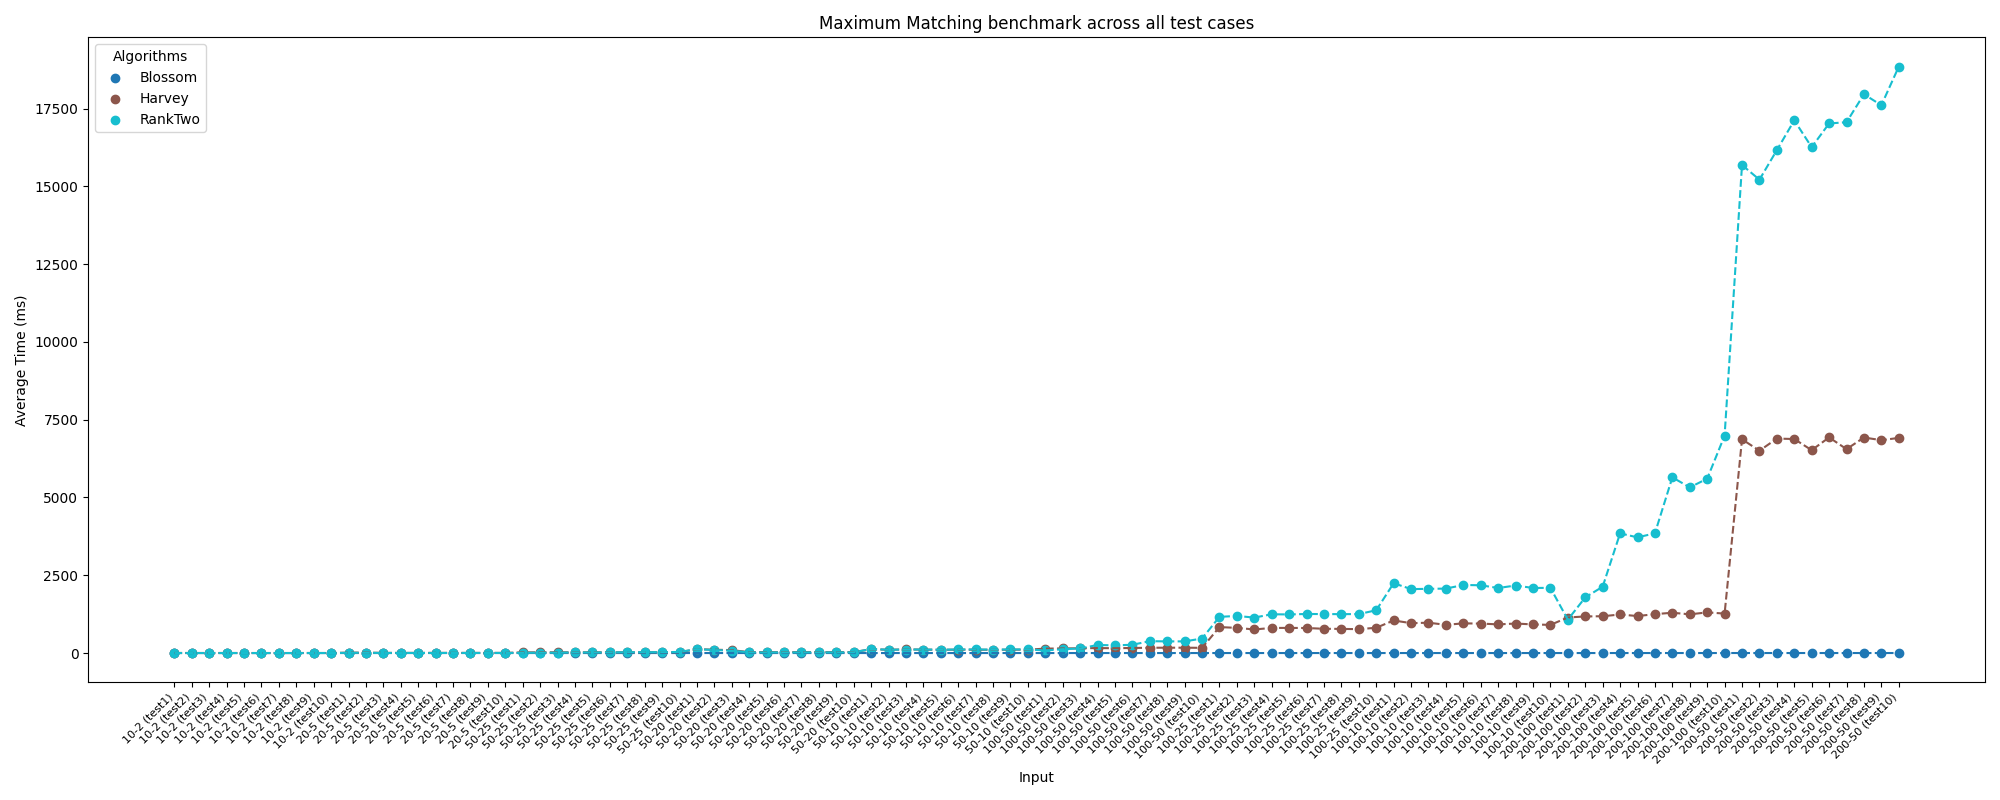
\includegraphics[width=15cm]{maximum_matching_plot.png}
  \caption{Maximum Matching benchmark with all test cases.}
  \label{fig:max_matching}
\end{figure}

Similarly to the perfect matching algorithm, in small graphs (\cref{fig:v10m2-v20m5}) the Rank-two algorithm outperforms the Harvey's algorithm.

\begin{figure}[H]
  \centering
  \begin{subfigure}{.5\textwidth}
    \centering
    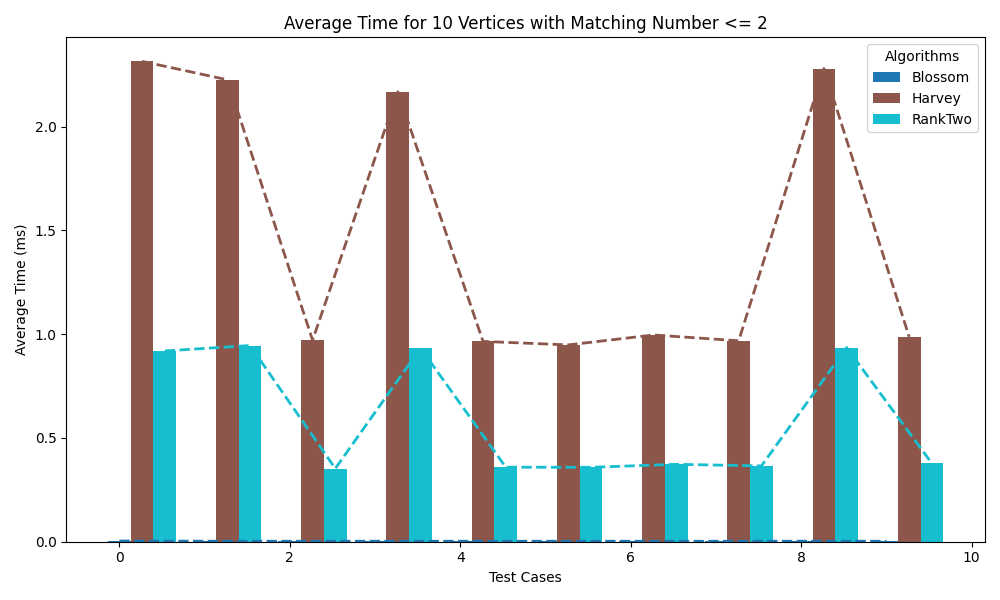
\includegraphics[width=\linewidth]{maximum_matching_v10_m2.png}
  \end{subfigure}%
  \begin{subfigure}{.5\textwidth}
    \centering
    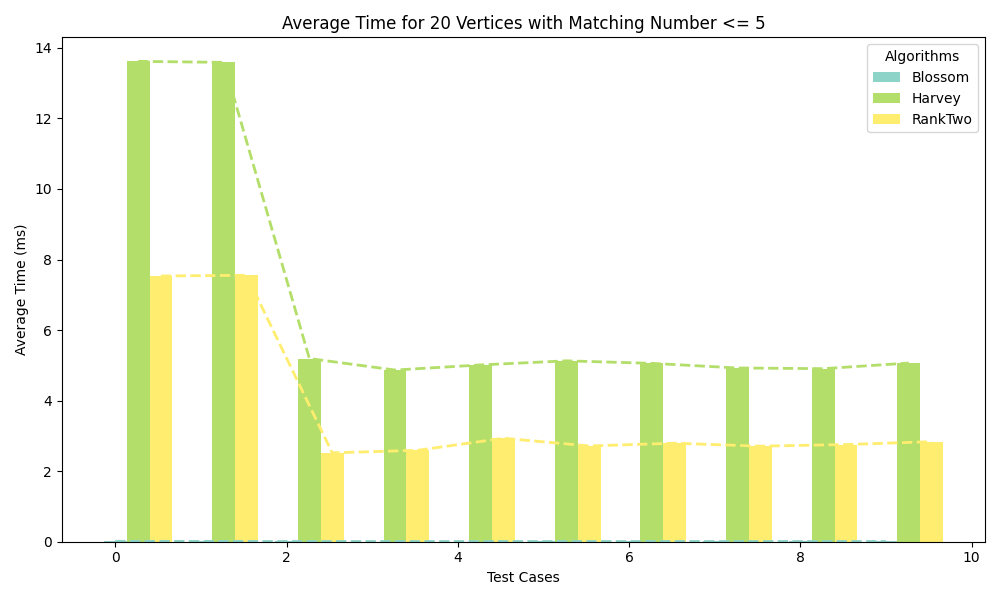
\includegraphics[width=\linewidth]{maximum_matching_v20_m5.png}
  \end{subfigure}
  \caption{Maximum matching benchmark with smaller graphs.}
  \label{fig:v10m2-v20m5}
\end{figure}

In \cref{fig:maxv50}, the impact of matching number on algorithm performance becomes evident through the augmented graph.
The left plot shows both algorithms maintaining stable, similar performance, likely due to the augmented graph's almost doubling the number of vertices.
Conversely, the right plot exhibits behavior reminiscent of the perfect matching algorithm, attributed to fewer added vertices in the augmented graph.

\begin{figure}[H]
  \centering
  \begin{subfigure}{.5\textwidth}
    \centering
    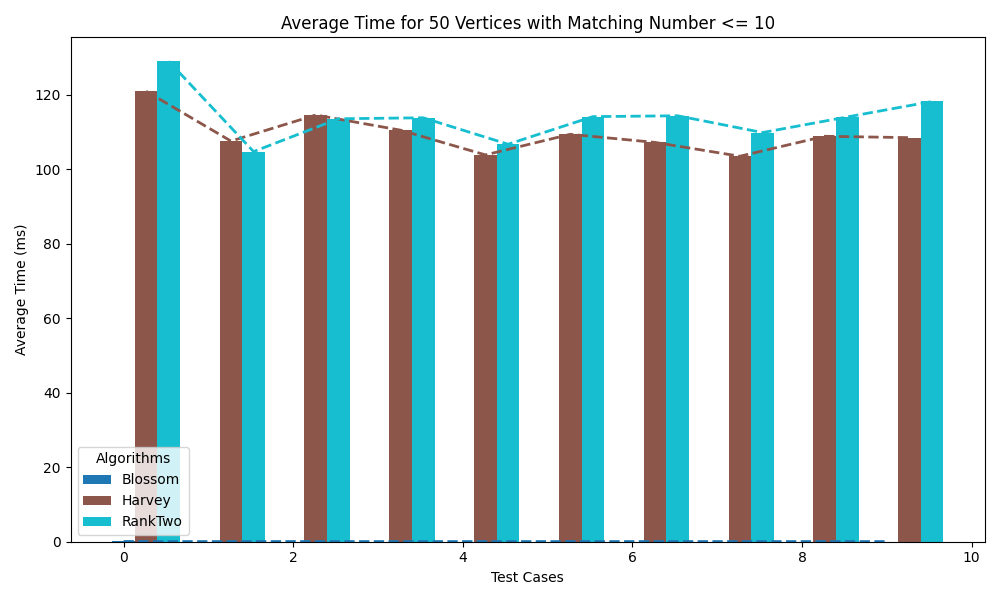
\includegraphics[width=\linewidth]{maximum_matching_v50_m10.png}
  \end{subfigure}%
  \begin{subfigure}{.5\textwidth}
    \centering
    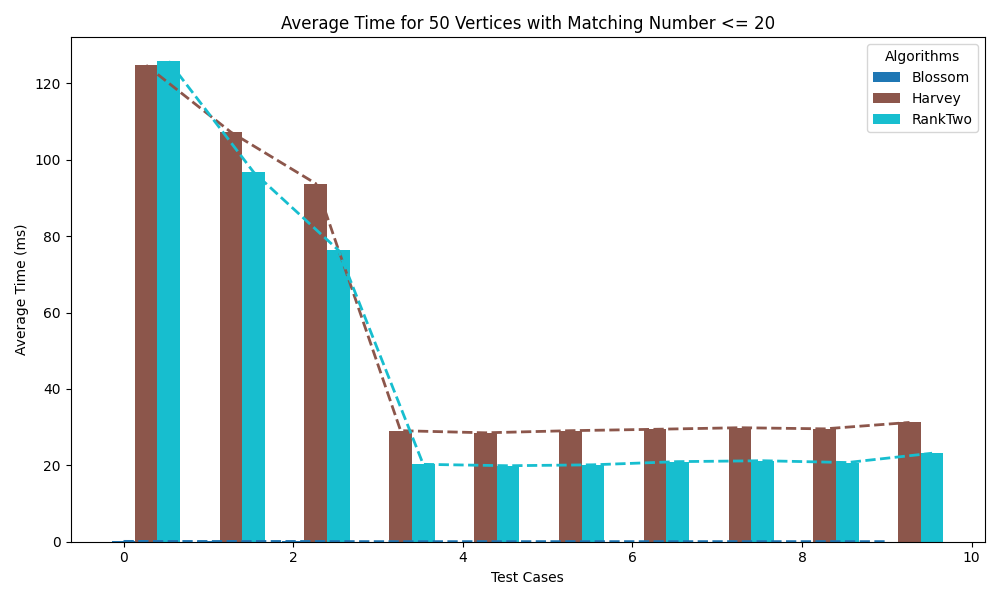
\includegraphics[width=\linewidth]{maximum_matching_v50_m20.png}
  \end{subfigure}
  \caption{Maximum matching benchmark with 50 vertices.}
  \label{fig:maxv50}
\end{figure}


In \cref{fig:maxv100} and \cref{fig:maxv200}, Harvey's algorithm outperforms the Rank-two algorithm.
The performance trend observed in \cref{fig:maxv50} recurs: as the graph's matching number increases, algorithm performance varies significantly due to augmented graph characteristics.

\begin{figure}[h]
  \centering
  \begin{subfigure}{.5\textwidth}
    \centering
    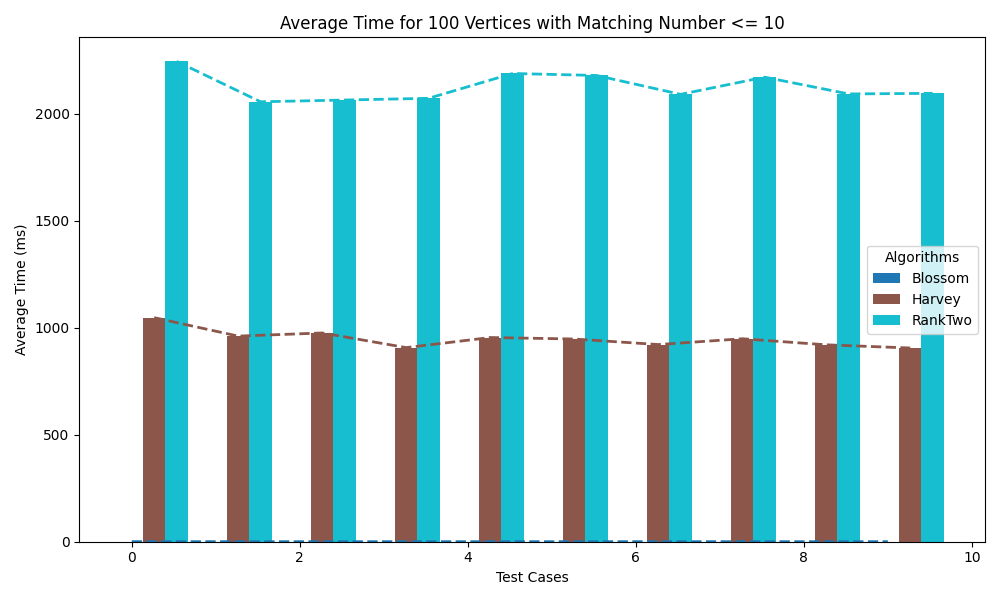
\includegraphics[width=\linewidth]{maximum_matching_v100_m10.png}
  \end{subfigure}%
  \begin{subfigure}{.5\textwidth}
    \centering
    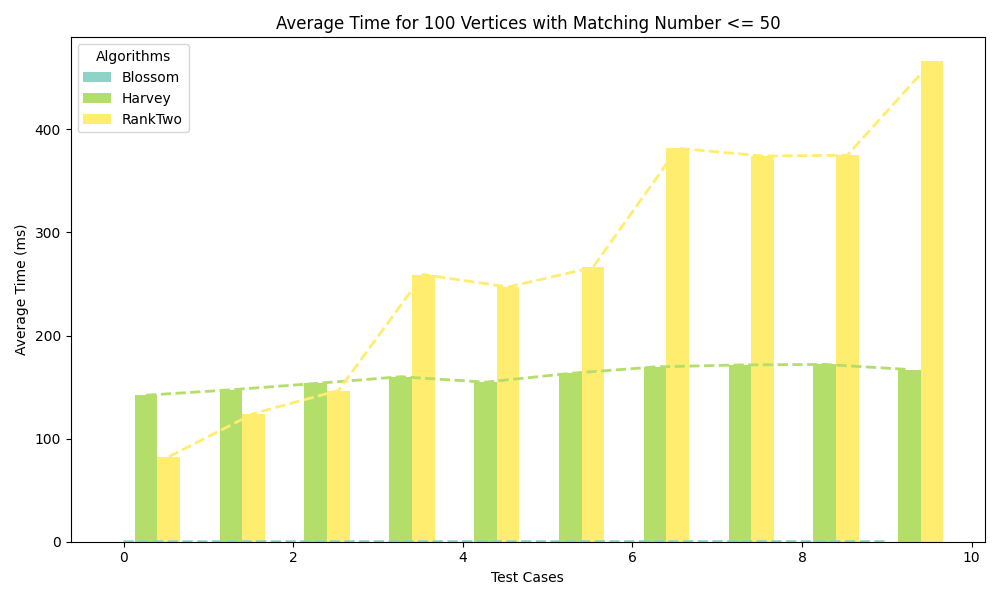
\includegraphics[width=\linewidth]{maximum_matching_v100_m50.png}
  \end{subfigure}
  \caption{Maximum matching benchmark with 100 vertices.}
  \label{fig:maxv100}
\end{figure}

\begin{figure}[h]
  \centering
  \begin{subfigure}{.5\textwidth}
    \centering
    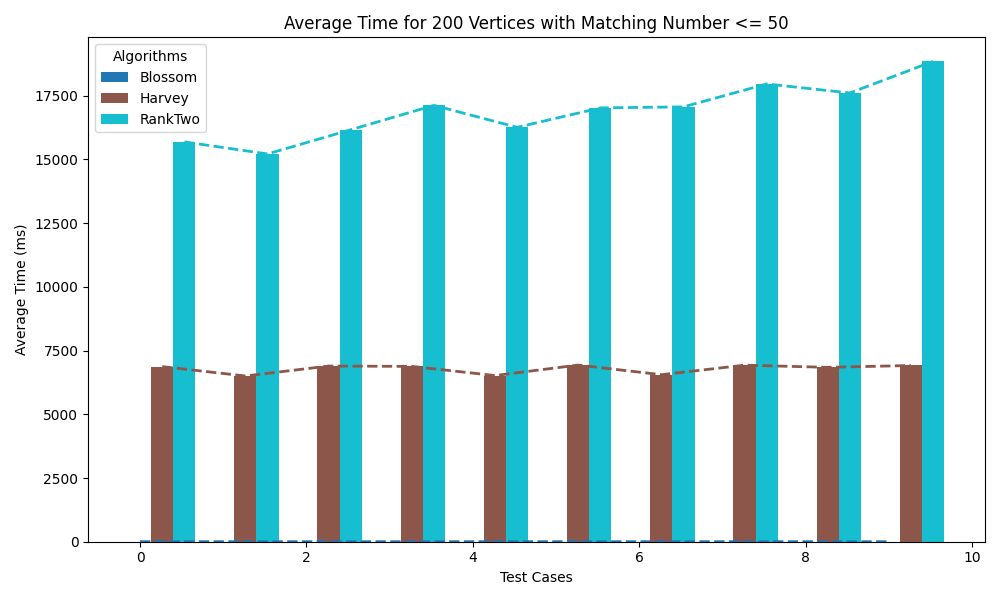
\includegraphics[width=\linewidth]{maximum_matching_v200_m50.png}
  \end{subfigure}%
  \begin{subfigure}{.5\textwidth}
    \centering
    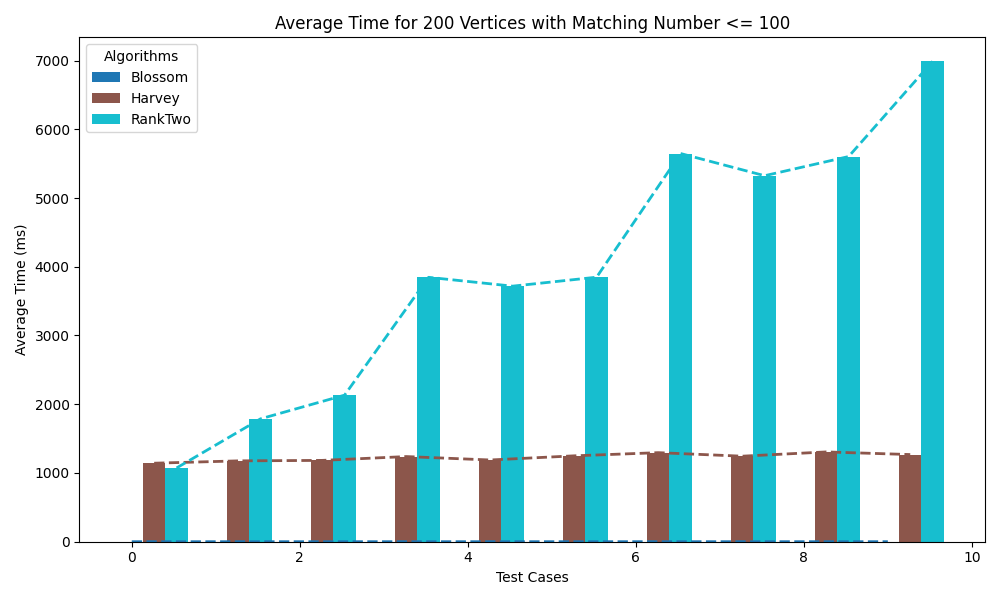
\includegraphics[width=\linewidth]{maximum_matching_v200_m100.png}
  \end{subfigure}
  \caption{Maximum matching benchmark with 200 vertices.}
  \label{fig:maxv200}
\end{figure}

% \begin{figure}[H]
%   \centering
%   \includegraphics[width=12cm]{boxplot_vX_mY.png}
%   \caption{Maximum Matching benchmark with X vertices and matching number Y.}
%   \label{fig:vXmY}
% \end{figure}

\chapter{Implementation}
\label{chap:implementation}

\section{Matrix implementation}
\label{sec:matrix_impl}

In this section, fundamental concepts related to matrix implementation are presented such as time complexity of various matrix operations,
matrix multiplication being as hard to compute as matrix inversion and others.
The objective is providing a sufficient understanding of key matrix operations.

\subsection{Definitions}

\begin{definition}[Schur complement]
    \label{def:schur}
    Let \(M\) be a square matrix of the form
    \[
        M = 
        \begin{pmatrix}
            W & X \\
            Y & Z 
        \end{pmatrix}
    \]
    where \(Z\) is a square matrix; Then, if \(Z\) is non-singular, the matrix
    \[
        C = W - X Z^{-1} Y
    \]
    is the \textit{Schur complement} of \(Z\) in \(M\).
\end{definition}

\subsection{Matrix operations}

\subsection{Matrix inverse}

An \(O(n^\omega)\) algorithm that computes the matrix inverse can be achieved exclusively using matrix multiplication with complexity \(O(n^\omega)\). 
The theorem and pseudo-code below demonstrates the process.

\begin{theorem}[Matrix inversions is no harder than matrix multiplication]
    \label{thm:mult_inv}
    If there is an algorithm that computes matrix multiplication in \(O(n^{\omega})\), then
    there is an algorithm that computes matrix inverse in \(O(n^{\omega})\).
\end{theorem}

\begin{proof}
    Theorem 28.2 from \citet{CLRS}.
\end{proof}

Now, the following algorithm can be implemented.
\begin{programruledcaption}{Matrix: \(\SC{Inverse}\)}
    \noindent
    \SC{Input:} A \(n \times n\) matrix \(A\) where \(n\) is a power of two; \\
    \SC{Output: } \(A^{-1}\). 

    \noindent \hrule
    \begin{lstlisting}[
      language={pseudocode},
      style=pseudocode,
      style=wider,
      functions={MatrixInverse},
      specialidentifiers={},
    ]
    function MatrixInverse(A) 
        if n = 1  
            if $A_{0, 0} = 0$ 
                // Matrix is singular.
            end
            $N_{0,0}$ := $1 / A_{0,0}$
            return N
        end
        $\begin{pmatrix} B & C \\ C^T & D\end{pmatrix}$ := A // Each submatrix size should be $n/2 \times n/2$.
        S := $D - CB^{-1}C^T$ // Schur complement (\ref{def:schur}).
        // Save results for $B^{-1}$ and $S^{-1}$.
        return $ \begin{pmatrix} B^{-1} + B^{-1}C^TS^{-1}CB^{-1} & -B^{-1}C^TS^{-1} \\ -S^{-1}CB^{-1} & S^{-1} \end{pmatrix}$ // \cref{thm:mult_inv}.
    end
    \end{lstlisting}
\end{programruledcaption}

\subsection*{Complexity}
Note that the algorithm above can be optimized to only calculate the recursive inversions a single time by saving them.
Suppose it is optimized.
Each call, has two recursive calls one for \(B^{-1}\) and another for \(S^{-1}\).
Suppose \(n = \max(n, m)\).
\begin{align}
    T(n) = O(n^2) + T(n/2, m/2) + O(n^2) + 2O(n^\omega) + 2T(n/2) + O(n^\omega)
\end{align}

\subsection{Matrix rank}
\input{content/07-analysis}

%%%%%%%%%%%%%%% SEÇÕES FINAIS (BIBLIOGRAFIA E ÍNDICE REMISSIVO) %%%%%%%%%%%%%%%%

% O comando backmatter desabilita a numeração de capítulos.
\backmatter

\pagestyle{backmatter}

% Espaço adicional no sumário antes das referências / índice remissivo
\addtocontents{toc}{\vspace{2\baselineskip plus .5\baselineskip minus .5\baselineskip}}

% A bibliografia é obrigatória

\printbibliography[
  title=\refname\label{sec:bib}, % "Referências", recomendado pela ABNT
  %title=\bibname\label{sec:bib}, % "Bibliografia"
  heading=bibintoc, % Inclui a bibliografia no sumário
]

\printindex % imprime o índice remissivo no documento (opcional)

\end{document}
